%\documentclass[compress,t,11pt]{beamer}
\documentclass[handout,compress,t,11pt]{beamer}
%\usetheme[sectionpage=none]{metropolis}           % Use metropolis theme
\usetheme[]{metropolis}           % Use metropolis theme
\usefonttheme{serif}
\definecolor[named]{Gray}{RGB}{111,112,114}
\definecolor[named]{DarkGray}{RGB}{48,48,48}
\definecolor[named]{Cardinal}{RGB}{179,22,34}
\usepackage[T1]{fontenc}
\usepackage[altbullet]{lucidabr}
\usepackage{textcomp}
\usepackage{upquote} % needed to make straight quotes work in listings
\usepackage{listgolang}
\usepackage{mathtools}
\usepackage{comment}
\usepackage{tikz}
\usepackage{tikzsymbols}
 \usetikzlibrary{trees,shapes,plotmarks,arrows,er,automata,petri,topaths,positioning}
\usepackage{pifont}
\usepackage{clrscode}
\usepackage{setspace}
\usepackage{soul}

\setbeamercolor{palette primary}{fg=white,bg=Cardinal}
\setbeamercolor{palette secondary}{fg=white,bg=Gray}
\setbeamercolor{palette tertiary}{fg=white,bg=Cardinal}
\setbeamercolor{palette quaternary}{fg=white,bg=Gray}
\setbeamercolor{palette sidebar primary}{fg=white,bg=Cardinal}
\setbeamercolor{palette sidebar secondary}{fg=white,bg=Gray}
\setbeamercolor*{titlelike}{fg=Cardinal}
\setbeamercolor{structure}{fg=Gray}
\setbeamercolor{title separator}{fg=Cardinal}
\setbeamercolor{alerted text}{fg=Cardinal}
\setbeamercolor{reversed}{fg=Cardinal,bg=black}

\newcommand{\card}[1]{\ensuremath{\left|#1\right|}}
\newcommand{\norm}[1]{\ensuremath{\|#1\|}}

\title[Programming in Go]{\bf Programming in Go}
\author{Matt Holiday} 
\institute[CP]{Cardinal Peak}
\date{20 March 2019} 
\subtitle{``In Go, the code does exactly what it says on the page''}
%\titlegraphic{\hfill\includegraphics[width=.25\textwidth,height=.25\textheight]{cp-logo-2x.png}}
\titlegraphic{
\begin{tikzpicture}[overlay, remember picture,scale=0.4]
\node[at=(current page.north east), anchor=north east] (a) {};
\node[below left = 0.1cm and 0.1cm of a] (b)
{\includegraphics[width=.25\textwidth,height=.25\textheight]{cp-logo-2x.png}};
\node[below left=2.56cm and 2.9cm of b]
{\includegraphics[width=.1\textwidth]{go-logo.png}};
\end{tikzpicture}}

\hypersetup{
    colorlinks=true,
    linkcolor=Cardinal,
    filecolor=magenta,      
    urlcolor=blue,
}

\setbeamerfont{footline}{series=\bfseries\selectfont}
\setbeamersize{text margin left=12pt,text margin right=12pt}
\linespread{1.0}
\metroset{block=fill}

\begin{document}
\frame{\titlepage} 

%\section{Introduction}
\begin{frame}
    \frametitle{A better C from the folks who created Unix \& C}
    {\setstretch{1.5} ``Go is more about software engineering than programming 
    lan-\\guage research. Or to rephrase, it is about language  design in the service of 
    software engineering.'' --- Rob Pike \\}
    \vspace{2\baselineskip}\par
    {\setstretch{1.5}``Go is not meant to innovate programming theory. It's meant to
    {\bf innovate programming practice}.'' --- Samuel Tesla \\}
    \vspace{3.4\baselineskip}
    \only<2>{``Go is like a better C, from the guys that didn't bring you C++'' \\
    --- Ikai Lan}
    
\end{frame}

\begin{frame}[fragile]
\frametitle{Hello, world!}
\begin{golang}
package main
import "fmt"

func main() {
    fmt.Println("Hello, world!")
}
\end{golang}
\end{frame}

\begin{frame}[fragile]
\frametitle{1, 2, 3, 5, 8, 13, 21, 34, 55, 89}
\begin{golang}
package main
import "fmt"

func fib() func() int {
	a, b := 0, 1

	return func() int {
		a, b = b, a+b
		return b
	}
}

func main() {
	f := fib()
	for x := f(); x < 100; x = f() {
		fmt.Println(x)
	}
}
\end{golang}
\end{frame}

\begin{frame}
    \frametitle{Why did they do it?}
    \vspace{0.6\baselineskip}
    \includegraphics[width=\textwidth,height=0.8\textheight]{mainframe-to-google.png}
    %\includegraphics[width=\textwidth,height=0.8\textheight]{server-room-interior-in-datacenter.jpg}
\end{frame}

\begin{frame}[fragile]
    \frametitle{Why did they do it?}
    A new language for a new computing landscape:
\begin{columns}
\begin{column}{0.5\textwidth}
    \vspace{-0.6\baselineskip}
    \begin{itemize}
    \item multicore processors
    \vspace{0.2\baselineskip}
    \item networked systems
    \vspace{0.2\baselineskip}
    \item massive clusters
    \vspace{0.2\baselineskip}
    \item the web programming model (think REST)
    \vspace{0.2\baselineskip}
    \item huge programs
    \vspace{0.2\baselineskip}
    \item large numbers of developers
    \vspace{0.2\baselineskip}
    \item long build times
    \vspace{0.2\baselineskip}
    \item C++ and Java don't fit that landscape well
    \end{itemize}
\end{column}
\begin{column}{0.45\textwidth}
\vspace{1.4\baselineskip}
\begin{table}[h!]
    % \caption{The 20th century rocks!}
    \begin{tabular}{r|l|l}
    \textbf{\#\#} & \textbf{Language} & \textbf{Year} \\
    \hline
    1 & JavaScript & 1995 \\
    2 & Java & 1995 \\
    3 & Python & 1991 \\
    4 & C\# & 2000 \\
    5 & C++ & 1983 \\
    6 & C & 1972 \\
    \end{tabular}
\end{table}
\end{column}
\end{columns}
%{\small Go is the \#1 language folks want to learn in 2018 \\(HackerRank 2019 Dev Skills Report).}
\end{frame}

\begin{frame}
    \frametitle{Why did they do it?}
    \vspace{0.6\baselineskip}
    \includegraphics[width=\textwidth,height=0.8\textheight]{40-years-processor-trend.png}
\end{frame}

\begin{frame}
    \frametitle{Why did they do it?}
    Pain points at Google:
    \begin{itemize}
    \item {\bf slow builds}
    \vspace{0.2\baselineskip}
    \item uncontrolled dependencies
    \vspace{0.2\baselineskip}
    \item each programmer using a {\bf different subset} of the language
    \vspace{0.2\baselineskip}
    \item poor program understanding (code hard to read, poorly documented, and so on)
    \vspace{0.2\baselineskip}
    \item duplication of effort
    \vspace{0.2\baselineskip}
    \item cost of updates
    \vspace{0.2\baselineskip}
    \item version skew
    \vspace{0.2\baselineskip}
    \item {\bf difficulty of writing static checkers \& other tools}
    \vspace{0.2\baselineskip}
    \item cross-language builds
    \end{itemize}
\end{frame}

\begin{frame}
    \frametitle{Built for Google's problems: Distributed systems}
    It's taking over the infrastructure/container/cloud world: \par
    \vspace{0.4\baselineskip}
    \begin{minipage}[c]{0.55\textwidth}
    \begin{itemize}
        \item Docker 
        \item Kubernetes
        \item Helm
        \item CoreOS (etcd, flannel)
        \item Prometheus 
        \item Grafana
        \item CockroachDB
        \item DropBox
        \item CloudFlare
    \end{itemize}
    \end{minipage}%
    \begin{minipage}[c]{0.35\textwidth}
        \vspace{0.5\baselineskip}
        \hfill \includegraphics[width=0.85\textwidth,height=.5\textheight]{gophers10th.jpg}
        \vspace{-1.2\baselineskip}
        \begin{center}\hspace{0.94in}{\tiny\textcopyright Ren\'ee French} \end{center}
    \end{minipage} \par
    \vspace{1.5\baselineskip}
    And I've delivered my first Go-based server to [redacted] ...
\end{frame}

\begin{frame}
    \frametitle{Design goals}
    Overall goals:
    \vspace{-0.2\baselineskip}
    \begin{itemize}
        \item \alert{\bf simplicity}, {\bf safety}, and {\bf readability}
        \item ease of expressing algorithms
        \item orthogonality
        \item one right way to do things
    \end{itemize}
    \vspace{1\baselineskip}
    Necessary, simple features with predictable behavior:
    \vspace{-0.2\baselineskip}
    \begin{itemize}
        \item interfaces \& methods
        \item packages
        \item concurrency
        \item tools \& build speed
    \end{itemize}
    \par \vspace{1.2\baselineskip}
    ``Clear is better than clever'' --- Go Proverb
\end{frame}
    %``A tool is in fact counterproductive when a large part 
    %of the entire project is taken up by mastering the tool.'' --- Niklaus Wirth

    % {\setstretch{1.2}``The leading principle and guideline was to produce a concep-\\
    % tionally simple language and to keep the number of features and
    % facilities minimal.'' --- Niklaus Wirth (regarding PL360) \\}

\begin{frame}
    \frametitle{Simplicity}
    \only<1-3>{A language with fewer features $\implies$ simplicity \par}
    \vspace{0.2\baselineskip}
    \only<1-3>{Simplicity $\implies$ readability $\implies$ reliability \& maintainability \par}

    \vspace{2\baselineskip}
    \only<2-3>{Think of {\em The Practice of Programming: \par}
    %\vspace{\baselineskip}
    \begin{minipage}[c]{0.45\textwidth}
        \begin{itemize}
            \item Simplicity
            \item Clarity
            \item Generality
        \end{itemize}
    \end{minipage}%
    \begin{minipage}[c]{0.45\textwidth}
        \hfill \includegraphics[width=.4\textwidth,height=.2\textheight]{pop-dog.png}
    \end{minipage} \par}
    \vspace{2\baselineskip}
    \only<3>{``If our basic tool,
      the language in which we design and code our programs, is also complicated,
      {\bf the language itself becomes part of the problem rather than part of its
      solution}.'' --- Tony Hoare}
    % \only<3>{``Users of UNIX will find that the most important characteristics of the
    % system are its {\bf simplicity, elegance, and ease of use}.'' \\
    % --- Ritchie \& Thompson (1974)}
\end{frame}

\begin{frame}
    \frametitle{Simplicity?}
    \begin{table}[h!]
        \begin{tabular}{llrr}
            C & {\tt \#include <stdio.h>} & 360 lines & 9 files \\
            C++ & {\tt \#include <iostream>} & 25326 lines & 131 files \\
            Go & {\tt import "fmt"} & 195 lines & 1 file\:\: \\
        \end{tabular}
    \end{table}    
    \begin{table}[h!]
        % \caption{The 20th century rocks!}
        \begin{tabular}{l||l|r|r}
        \textbf{Language} & \textbf{Year} & \textbf{Keywords} & \textbf{Pages} \\
        \hline \hline
        Pascal     & 1974     & 35 & 167  \\
        \hline
        ANSI C     & 1988     & 32 & 238  \\
        C11        & 2011     & 44 & 683  \\
        \hline
        C++        & 1990     & 48 & 480  \\
        C++14      & 2014     & 86 & 1330 \\
        \hline
        Java 8     & 2015     & 50 & 788  \\
        \hline
        Go         & 2012     & 25 & 98   \\
        \end{tabular}
    \end{table}
    \center{C++20 may well be as big a release as C++11; draft over 1700 pp.}
\end{frame}

\begin{frame}
    \frametitle{Odious comparisons}
    My subjective take:
    \begin{itemize}
    \item Go is as fast as Java and faster than interpreted languages
    \item with more safety but still very easy to use
    \item and offers radical simplicity
    \end{itemize}

    \vspace{\baselineskip}
    {\bf YMMV}:
    \vspace{-1.62\baselineskip}
    \begin{table}[h!]
        \begin{tabular}{l||r|r|r}
        \textbf{Language}& \textbf{Safety} & \textbf{Ease} & \textbf{Speed}  \\
        \hline \hline
        Go           & 9 & 8 & 7  \\
        \hline
        Java / C\#   & 7 & 6 & 6  \\
        \hline
        Python       & 5 & 9 & 1  \\
        \hline
        Javascript   & 5 & 7 & 2  \\
        \hline
        C++          & 3 & 5 & 8  \\
        \hline
        C            & 1 & 3 & 9  \\
        \end{tabular}
    \end{table}
    \vspace{0.4\baselineskip}
    ``Fast languages aren't safe, easy-to-use languages aren't fast''
\end{frame}


% \begin{frame}
%     \frametitle{KISS}
%     {\setstretch{1.2} ``The price of reliability is the pursuit of the utmost
%     simplicity.'' \\--- Tony Hoare}
%     \par \vspace{1.5\baselineskip}
%     {\setstretch{1.3} ``Simplicity is a great virtue but it requires hard work
%     to achieve \\it and education to appreciate it. And to make matters worse:
%     {\bf complexity sells better}.'' --- Edsger Dijkstra \\}
%     \par \vspace{3.5\baselineskip}
%     \only<2>{{\em The Problem With Software: Why Smart Engineers Write Bad Code} \par
%     \par \vspace{0.5\baselineskip}
%     {\em A Philosophy of Software Design}}
% \end{frame}

% \begin{frame}
%     \frametitle{OK, one more Tony Hoare quote}
%      \vspace{\baselineskip}
%      {\setstretch{1.5}{``It therefore seems especially necessary in the design of a
%       new programming language . . . to \alert{{\bf\em pursue the goal of simplicity
%       to an extreme}}, so that a programmer can readily  learn and
%       remember all its features, can select the best facility for each of his
%       purposes, can \alert{{\bf\em fully understand the effects and consequences of
%       each decision},} and can then concentrate the major part of his intellectual
%        effort to \alert{{\bf\em understanding  his problem and his programs rather
%         than his tool}.}'' \\}}
%       \par \vspace{0.5\baselineskip}
%       \hfill {\em Hints on Programming Language Design} (1973) \hspace{0.24in}
% \end{frame}

% \begin{frame}
%     \frametitle{OK, one more quote}
%      \vspace{0.4\baselineskip}
%      {\setstretch{1.5}{``Programmers are always surrounded by complexity; we cannot avoid it.
%       Our applications are complex because we are ambitious to use our computers in ever
%       more sophisticated ways. Programming is complex because of the large number of
%       conflicting objectives for each of our programming projects. If our basic tool,
%       the language in which we design and code our programs, is also complicated,
%       \alert{{\bf the language itself becomes part of the problem rather than part of its
%       solution}.}'' --- Tony Hoare \\}}
%       \par \vspace{\baselineskip}
%       \hfill {\em The Emperor's Old Clothes} (Turing Award Lecture, 1980) \hspace{0.03in}
% \end{frame}


% \begin{frame}
%     \frametitle{OK, two more Tony Hoare quotes}
%      \vspace{\baselineskip}
%      {\setstretch{1.5}{``There are two ways of constructing a software design: One way
%      is to make it so simple that there are {\em obviously} no deficiencies and the other way
%      is to make it so complicated that there are no {\em obvious} deficiencies.'' \\}}
%       \par \vspace{0.5\baselineskip}
%       \hfill {\em The Emperor's Old Clothes} (Turing Award Lecture, 1980) \hspace{0.06in}
% \end{frame}

% \begin{frame}
%     \frametitle{And another from Edsger Dijkstra}
%      \vspace{\baselineskip}
%      {\setstretch{1.5}{``We shall do a much better programming job, provided that we
%      approach the task with a full appreciation of its tremendous dif-\\ficuly, provided
%      that we stick to modest and elegant programming languages, provided that we
%      respect the intrinsic limitations of the human mind, and approach the task as
%      Very Humble Programmers.'' \\}}
%       \par \vspace{0.5\baselineskip}
%       \hfill {\em The Humble Programmer} (Turing Award Lecture, 1972) \hspace{0.06in}
% \end{frame}

% Algol W is a relatively clean language which presents the new programmer with a minimum 
% number of magical phrases which must simply be accepted until they can be explained 
% later. --- Daniel Boulet


% \begin{frame}
% \frametitle{Once more, with feeling}
% {\setstretch{1.5}{
% ``PL/1 {\em [etc., etc.]} has a huge variety of language features designed to satisfy the
% needs of a large class of programmers. Although each of these features may be very attractive
% on its own, the complexity of the language as a whole is so high that {\bf mastering the
% complete  language becomes a real problem}. One of the main lessons to be learned from this
% experience is that {\bf the complexity of a language can affect the readability, verifiability
% and maintenance of its programs}.'' --- Johan Lewi \& Jan Paredaens\\}}\par
% \vspace{\baselineskip}
% (from {\em Data Structures in Pascal, Algol 68, PL/1 and Ada})
% \end{frame}

\section{What It Is}
\begin{frame}
    \frametitle{Static but easy typing}
    \only<1-2>{{\setstretch{1.5} ``Go is an attempt to combine the ease of programming 
    of an interpreted, dynamically typed language with the efficiency and safety of
    a statically typed, compiled language.'' --- {\em Go FAQ} \par}}
    
    % \vspace{3.6\baselineskip}
    % \only<2-2>{``When there is no type hierarchy you don't have to manage the \\%
    % type hierarchy.'' --- Rob Pike \par}
    % \only<2>{{\setstretch{1.2}``I've been experimenting with moving C code to Go over
    % the last week, and I'm noticing two things. One is that it's easy to do;
    % C's idioms map over pretty well. The other is that {\bf the resulting code \\
    % is much simpler}.'' --- ESR, ``The big break in computer languages'' \par
    \vspace{8\baselineskip}
    \only<2-2>{``Clumsy type systems drive people to dynamically typed languages.'' --- Robert Griesemer}
\end{frame}

\begin{frame}[fragile]
\frametitle{Look, Ma, no types!}
\begin{golang}
package main
import ("io"; "log"; "os")

func main() {
    for _, fname := range os.Args[1:] {
        file, err := os.Open(fname)

        if err != nil {
            log.Fatal(err)
        }

        if _, err = io.Copy(os.Stdout, file); err != nil {
            log.Fatal(err)
        }
        
        file.Close()
    }
}
\end{golang}
\end{frame}

\begin{frame}
    \frametitle{Concurrency based on Tony Hoare's CSP}
    Communicating sequential processes \par
    \vspace{\baselineskip}
    Break your program into ``nanoservices'' that talk to each other \par
    \vspace{\baselineskip}
    Like Erlang, but Go's channel model is more flexible and natural \par
    \vspace{3\baselineskip}
    \only<2>{{\setstretch{1.3} ``Go doesn't force developers to embrace the asynchronous 
    ways of event-driven programming. ... That lets you {\bf write asynchronous code 
    in a synchronous style}. As people, we're much better suited to writing about 
    things in a synchronous style.'' --- Andrew Gerrand \\}}
    % {\setstretch{1.3} ``CSP [Communicating sequential processes] has the property
    % that it's easy to add to a procedural programming model without pro-\\found changes
    % to that model.'' --- Rob Pike \\}
\end{frame}

\begin{frame}
    \frametitle{Go's Concurrency Features}
    \only<1-4>{Goroutines --- lightweight coroutines multiplexed onto threads \par}
    \vspace{\baselineskip}
    \only<2-4>{Channels (similar to shell pipes in Unix) \par}
    \vspace{\baselineskip}
    \only<3-4>{A {\tt select} block allows multiplexing channels {\em in source code} \par}
    \vspace{4\baselineskip}
    \only<4>{Think of channels as vehicles to transfer ownership \par}
    \vspace{\baselineskip}
    \only<4>{``Don't communicate by sharing memory; instead, {\bf share memory by 
    communicating}.'' --- Rob Pike}
\end{frame}

\begin{frame}[fragile]
\frametitle{Concurrency Example 1: Channels}
\begin{golang}
results := make(chan int)

// asynchronously yield a stream of integers

go func(limit int, out chan<- int) {
    for i := 0; i < limit; i++ {
        out <- i
    }

    close(out)  // else we would deadlock
}(10, results)

// receive them when they're ready

for i := range results {
    fmt.Println(i)
}
\end{golang}
\end{frame}

\begin{frame}[fragile]
\frametitle{Concurrency Example 2: Stream of IDs}
\begin{golang}
var nextID = 0

func handler(w http.ResponseWriter, r *http.Request) {
    fmt.Fprintf(w, "<h1>You got %v<h1>", nextID)

    // unsafe - data race

    nextID++
}

func main() {
    http.HandleFunc("/", handler)
    if err := http.ListenAndServe(":8080", nil); err != nil {
        log.Fatal(err)
    }
}

// simple HTTP server example from Francesc Campoy
\end{golang}
\end{frame}

\begin{frame}[fragile]
\frametitle{Concurrency Example 2: Stream of IDs}
\begin{golang}
var nextID = make(chan int)

func handler(w http.ResponseWriter, q *http.Request) {
    fmt.Fprintf(w, "<h1>You got %v<h1>", <-nextID)
}

func counter() {
    for i := 0; ; i++ {
        nextID <- i
    }
}

func main() {
    go counter()
    http.HandleFunc("/", handler)
    if err := http.ListenAndServe(":8080", nil); err != nil {
        log.Fatal(err)
    }
}
\end{golang}
\end{frame}

\begin{frame}[fragile]
    \frametitle{Concurrency Example 3: Prime Sieve}
    \vspace{0.4\baselineskip}
    \only<1-4>{\begin{center}
        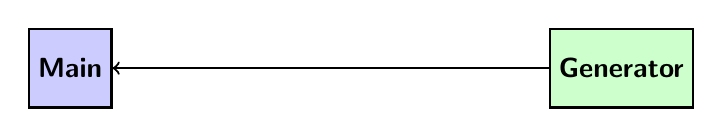
\begin{tikzpicture}[scale=0.5]            
            \tikzstyle{state}=[rectangle,minimum size=1cm,font=\sffamily\bfseries,draw]
            \tikzstyle{link}=[font=\sffamily\bfseries]

            \tikzstyle{every edge}=[thick,draw]

            \tikzstyle{M}=[state,thick,fill=green!20]    % main graph
            \tikzstyle{A}=[state,thick,fill=blue!20]     % clique
            \tikzstyle{C}=[state,thick,fill=red!20]      % key node

            \node[A] (0) at (-1, 0) {Main};
            \node[M] (4) at (13, 0) {Generator};

            \tikzstyle{E}=[ultra thick,color=red]  % min cut

            \path[<-] (0) edge (4);
        \end{tikzpicture}
    \end{center}}

    \only<2-4>{\begin{center}
        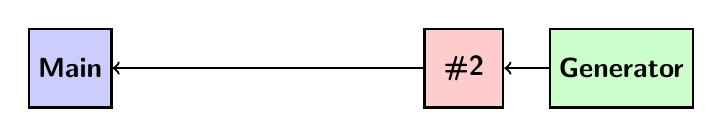
\begin{tikzpicture}[scale=0.5]            
            \tikzstyle{state}=[rectangle,minimum size=1cm,font=\sffamily\bfseries,draw]
            \tikzstyle{link}=[font=\sffamily\bfseries]

            \tikzstyle{every edge}=[thick,draw]

            \tikzstyle{M}=[state,thick,fill=green!20]    % main graph
            \tikzstyle{A}=[state,thick,fill=blue!20]     % clique
            \tikzstyle{C}=[state,thick,fill=red!20]      % key node

            \node[A] (0) at (-1, 0) {Main};
            \node[C] (3) at ( 9, 0) [align=center]{\#2};
            \node[M] (4) at (13, 0) {Generator};

            \tikzstyle{E}=[ultra thick,color=red]  % min cut

            \path[<-] (0) edge (3);
            \path[<-] (3) edge (4);
        \end{tikzpicture}
    \end{center}}
    
    \only<3-4>{\begin{center}
        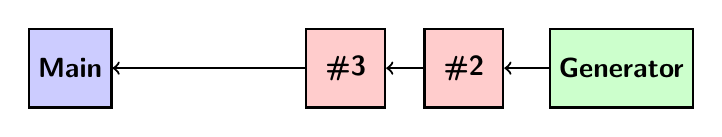
\begin{tikzpicture}[scale=0.5]            
            \tikzstyle{state}=[rectangle,minimum size=1cm,font=\sffamily\bfseries,draw]
            \tikzstyle{link}=[font=\sffamily\bfseries]

            \tikzstyle{every edge}=[thick,draw]

            \tikzstyle{M}=[state,thick,fill=green!20]    % main graph
            \tikzstyle{A}=[state,thick,fill=blue!20]     % clique
            \tikzstyle{C}=[state,thick,fill=red!20]      % key node

            \node[A] (0) at (-1, 0) {Main};
            \node[C] (2) at ( 6, 0) [align=center]{\#3};
            \node[C] (3) at ( 9, 0) [align=center]{\#2};
            \node[M] (4) at (13, 0) {Generator};

            \tikzstyle{E}=[ultra thick,color=red]  % min cut

            \path[<-] (0) edge (2);
            \path[<-] (2) edge (3);
            \path[<-] (3) edge (4);
        \end{tikzpicture}
    \end{center}}

    \only<4>{\begin{center}
        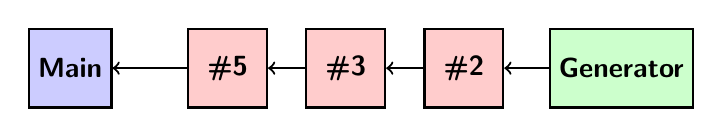
\begin{tikzpicture}[scale=0.5]            
            \tikzstyle{state}=[rectangle,minimum size=1cm,font=\sffamily\bfseries,draw]
            \tikzstyle{link}=[font=\sffamily\bfseries]

            \tikzstyle{every edge}=[thick,draw]

            \tikzstyle{M}=[state,thick,fill=green!20]    % main graph
            \tikzstyle{A}=[state,thick,fill=blue!20]     % clique
            \tikzstyle{C}=[state,thick,fill=red!20]      % key node

            \node[A] (0) at (-1, 0) {Main};
            \node[C] (1) at ( 3, 0) [align=center]{\#5};
            \node[C] (2) at ( 6, 0) [align=center]{\#3};
            \node[C] (3) at ( 9, 0) [align=center]{\#2};
            \node[M] (4) at (13, 0) {Generator};

            \tikzstyle{E}=[ultra thick,color=red]  % min cut

            \path[<-] (0) edge (1);
            \path[<-] (1) edge (2);
            \path[<-] (2) edge (3);
            \path[<-] (3) edge (4);
        \end{tikzpicture}
    \end{center}}
\end{frame}

\begin{frame}[fragile]
\frametitle{Concurrency Example 3: Prime Sieve}
\begin{golang}
// Doug McIlroy (1968) via Tony Hoare (1978)
// code example from the Go language spec

func generate(limit int, ch chan<- int) {
    for i := 2; i < limit ; i++ {
        ch <- i
    }
    close(ch)
}

func filter(src <-chan int, dst chan<- int, prime int) {
    for i := range src {
        if i % prime != 0 {
            dst <- i
        }
    }
    close(dst)
}
\end{golang}
\end{frame}

\begin{frame}[fragile]
\frametitle{Concurrency Example 3: Prime Sieve}
\begin{golang}
func sieve(limit int) {
    ch := make(chan int)
    go generate(limit, ch)
    for {
        prime, ok := <- ch
        if !ok {
            break
        }
        ch1 := make(chan int)
        go filter(ch, ch1, prime)
        ch = ch1
        fmt.Print(prime, " ")
    }
}

func main() {
    sieve(100) // 2 3 5 7 11 13 17 19 23 29 31 37 41 43 ... 
}
\end{golang}
\end{frame}

% \begin{frame}[fragile]
%     \frametitle{Concurrency Example 4: Select}
%     Select allows composing channels in ways that mutexes can't \par
%     \vspace{0.5\baselineskip}
% \begin{golang}
% for {
%     select {
%     case frame := <-n.Input:
%         . . .
%
%     case <-n.Ctx.Done():
%         // cancellation
%         _ = n.handler.Handle(&Result{err: n.Ctx.Err()})
%         return
%
%     case <-time.After(30 * time.Second):
%         // timeout
%         _ = n.handler.Handle(&Result{err: timeout})
%         return
%     }
% }
% \end{golang}
% \end{frame}


% \begin{frame}[fragile]
% \frametitle{Concurrency Example 2: Sieve of Eratosthenes}
% \begin{golang}
% // https://siongui.github.io/2017/04/17/go-sieve-of-eratosthenes/
% func SieveOfEratosthenes(n int) []int {
%     // All ints prime until they're found to be not prime
%     ints := make([]bool, n+1)
%     for i := 2; i < n+1; i++ {
%         ints[i] = true
%     }
%
%     for p := 2; p*p <= n; p++ {
%         // If ints[p] is not changed, then it is a prime
%         if ints[p] {
%             // Update all the multiples of p
%             for i := p * 2; i <= n; i += p {
%                 ints[i] = false
%             }
%         }
%     }
%
%     . . .
% \end{golang}
% \end{frame}
%
% \begin{frame}[fragile]
% \frametitle{Concurrency Example 2: Sieve of Eratosthenes}
% \begin{golang}
%     . . .
%
%     var primes []int
%
%     // return all prime numbers <= n
%     for p := 2; p <= n; p++ {
%         if ints[p] {
%             primes = append(primes, p)
%         }
%     }
%
%     return primes
% }
% \end{golang}
% What it looks like in APL: \:\:\:
% \raisebox{-0.3\height}{\includegraphics[width=.5\textwidth,height=.1\textheight]{apl-sieve.png}}
% \end{frame}

% \begin{frame}[fragile]
% \frametitle{Concurrency Example 2: Prime Sieve Alernative}
% \begin{golang}
% func sieve(limit int) {
%     c := make(chan int)
%     ch := &c
%     go generate(limit, *ch)
%     for p := range *ch {  // use range on ptr to chan
%         fmt.Print(p, " ")
%         ch1 := make(chan int)
%         go filter(*ch, ch1, p)
%         *ch = ch1
%     }
% }
% \end{golang}
% \end{frame}

% \begin{frame}[fragile]
% \frametitle{Concurrency Example 3: Select}
% \begin{golang}
% odds := make(chan int)
% evens := make(chan int)
%
% go func() {
%     for i := 0; i < 12; i++ {
%         if j := rand.Intn(32); j % 2 == 1 {
%             odds <- j
%         } else {
%             evens <- j
%         }
%     }
%
%     close(odds)
%     close(evens)
% }()
%
% . . .
% \end{golang}
% \end{frame}
% \begin{frame}[fragile]
% \frametitle{Concurrency Example 3: Select}
% \begin{golang}
% . . .
%
% for evens != nil && odds != nil {
%     select {
%         case i, ok := <-odds:
%             if ok {
%                 fmt.Printf("odd %v\n", i)
%             } else {
%                 odds = nil
%             }
%         case j, ok := <-evens:
%             if ok {
%                 fmt.Printf("even %v\n", j)
%             } else {
%                 evens = nil
%             }
%     }
% }
% \end{golang}
% \end{frame}

\begin{frame}
    \frametitle{Object-orientation based loosely on Oberon-2}
    \only<1-4>{Type-bound functions (methods) {\em on any named type} \par}
    \vspace{\baselineskip}
    \only<2-4>{Abstraction using interfaces \par}
    \vspace{\baselineskip}
    \only<3-4>{Encapsulation using packages \par}
    \vspace{\baselineskip}
    \only<4>{Composition not inheritance \par}
 
    % \only<1-5>{Composition (has-a) --- {\bf not} inheritance (is-a) \par
    % \vspace{\baselineskip}
    % \only<2-5>{Type-bound functions (methods) {\em on any type} \par}
    % \vspace{\baselineskip}
    % \only<3-5>{Interfaces $\implies$ protocol-oriented programming \par}
    % \vspace{\baselineskip}
    % \only<4-5>{Duck-typing for interface conformance \par
    \vspace{4.5\baselineskip}
    \only<4>{``{\bf Prefer composition to inheritance}'' \\ --- Joshua Bloch, 
    {\em Effective Java}}
\end{frame}

\begin{frame}[fragile]
    \frametitle{Object-Oriented Example 1: Interfaces}
\begin{golang}
type Stringer interface { // pre-declared in Go
    String() string
}

type Pair struct {
    Path string
    Hash string
}

func (p Pair) String() string {
	return fmt.Sprintf("Hash of %v is %v", p.Path, p.Hash)
}

p := Pair{"/usr", "0xfdfe"}

fmt.Println(p) // calls p.String() automatically
               // "Hash of /usr is 0xfdfe"
\end{golang}
\end{frame}

\begin{frame}[fragile]
    \frametitle{Object-Oriented Example 1: Interfaces}
\begin{golang}
// Sizer describes the Size() method that gets the
// total size of an item. [Mat Ryer]

type Sizer interface {
    Size() int64
}

func (f *File) Size() int64 {
    return f.info.Size()
}

func Fits(capacity int64, s Sizer) bool {
    return capacity > s.Size()
}

func IsEmailable(s Sizer) bool {
    return s.Size() < 1<<20
}
\end{golang}
\end{frame}

\begin{frame}[fragile]
    \frametitle{Object-Oriented Example 1: Interfaces}
\begin{golang}
// add the ability to pass a slice of Sizers to Fits

type Sizers []Sizer

func (s Sizers) Size() int64 {
    var total int64

    for _, sizer := range s {
        total += sizer.Size()
    }

    return total
}

f1 := new(File) // returns *File
f2 := new(File)
ok := Fits(42, Sizers{f1, f2})
\end{golang}
\end{frame}

% \begin{frame}[fragile]
%     \frametitle{Object-Oriented Example 2: Interfaces}
% \begin{golang}
% type Result interface {
%     Name() stage
%     Value() []byte
% }
%
% type asrResult struct {
%     stage stage
%     text  string
% }
%
% func (r asrResult) Name() state { return r.stage }
%
% func (r asrResult) Value() []byte {
%     if r.stage == EOS {
%         return []byte(fmt.Sprintf(`"partial":"%s"`, r.text))
%     }
%     return []byte(fmt.Sprintf(asrDetail, r.text, r.conf))
% }
% \end{golang}
% \end{frame}
%
% \begin{frame}[fragile]
%     \frametitle{Object-Oriented Example 2: Interfaces}
% \begin{golang}
% type nluResult struct {
%     intent  string
%     score   float32
%     missing nluError
% }
%
% var nluOK = `"NLU": {"intentName":"%s", "score":%.2f}`
% var nluFailed = `"NLU": {"intentName":"%s", "missing":"%s"}`
%
% func (r nluResult) Name() state { return NLU }
%
% func (r nluResult) Value() []byte {
%     if r.missing == noError {
%         return []byte(fmt.Sprintf(nluOK, r.intent, r.score))
%     }
%     return []byte(fmt.Sprintf(nluFailed, "sorry", r.missing))
% }
% \end{golang}
% \end{frame}

% \begin{frame}[fragile]
%     \frametitle{Object-Oriented Example 2: Composition}
% \begin{golang}
% type Pair struct {
%     Path string
%     Hash string
% }
%
% type PairWithLength struct {
%     Pair
%     Length int
% }
%
% // construction requires explicit sub-parts
% // then we get direct access Pair parts/methods
%
% pl := PairWithLength{Pair{"/usr", "0xfdfe"}, 121}
%
% fmt.Println(pl.Path, pl.Length)
% fmt.Println(pl.String())        // "Hash of /usr is 0xfdfe"
% \end{golang}
% \end{frame}

\begin{frame}[fragile]
    \frametitle{Object-Oriented Example 2: Composition}
\begin{golang}
type Reader interface {
    Read(p []byte) (n int, err error)
}

type Writer interface {
    Write(p []byte) (n int, err error)
}

type ReadWriter interface {
    Reader
    Writer
}

// one of several ways to do this, all equal
type ReadWriteCloser interface {
    ReadWriter
    Close() error
}
\end{golang}
\end{frame}
\begin{frame}[fragile]
\frametitle{Object-Oriented Example 2: Composition}
\begin{golang}
func handler(w http.ResponseWriter, r *http.Request) {
    f, err := os.Open("./static/" + path.Base(r.URL.Path))

    if err != nil {
        http.Error(w, err.Error(), 404)
        return
    }


    // func Copy(dst Writer, src Reader) (int64, error)

    _, err := io.Copy(w, f)

    if err != nil {
        http.Error(w, err.Error(), 500)
    }
}
\end{golang}
\end{frame}

\begin{frame}
    \frametitle{Fast compiles, small binaries, and lots of tools}
    \only<1-3>{Packages carry transitive import data $\implies$ fast compiles \\
    \vspace{0.3\baselineskip}
    ({\bf no} include [re]-pre-processing as in C) \par}
    \vspace{\baselineskip}
    \only<2-3>{Statically-linked binaries $\implies$ tiny, safe containers \par}
    \vspace{\baselineskip}
    \only<3-3>{The language supports static analysis well:
    \begin{itemize}
        \item standard source formatting
        \item library includes all front-end parsing software
    \end{itemize}
    \vspace{0.8\baselineskip}
    Built-in tools include:
    \begin{itemize}
        \item check style \& correctness (golint, go vet)
        \item fetch 3rd-party packages (go get)
        \item generate documentation (go doc)
    \end{itemize}}
\end{frame}

\begin{frame}[fragile]
    \frametitle{The compiler gives no warnings}
    Strictness $\implies$ less ambiguity $\implies$ fewer misteaks\par
        \vspace{0.4\baselineskip}
    \begin{minipage}[c]{0.55\textwidth}
    \begin{itemize}
        \item braces are required for {\bf all} control statements
        \vspace{0.4\baselineskip}
        \item no unused imports or variables
        \vspace{0.4\baselineskip}
        \item no automatic integer/boolean conversions
        \vspace{0.4\baselineskip}
        \item switch cases don't fall through by default
        \vspace{0.4\baselineskip}
        \item assignment \& increment are statements, not expressions
    \end{itemize}
    \end{minipage}%
    \begin{minipage}[c]{0.35\textwidth}
        \hfill \includegraphics[height=.45\textheight]{black-hat-go.png}
    \end{minipage} \par
    \vspace{1\baselineskip}
    ``{\bf Form is liberating}'' --- quoted in {\em The Mythical Man-Month} 
\end{frame}

\begin{frame}[fragile]
    \frametitle{What else?}
    \only<1-2>{{\bf Garbage collection} \par}
    \vspace{\baselineskip}
    \only<1-2>{Built-in race detector for testing \par}
    \vspace{\baselineskip}
    \only<1-2>{Unicode support (Go source is UTF-8) \par}
    \vspace{\baselineskip}
    \only<1-2>{Easy encode/decode of JSON, etc. using {\em reflection} \par}
    \vspace{\baselineskip}
    \only<1-2>{Tools and ``unsafe'' operations for interfacing to C (cgo) \par}
    \vspace{1.6\baselineskip}
    \only<2>{{\bf A standard for code formatting supported by tools!} \\
    (\st{brace wars})}
\end{frame}

\begin{frame}[fragile]
    \frametitle{What else?}
    No runtime dependencies:
    \begin{itemize}
        \item no interpreter or JVM
        \item if pure Go, no \verb|libc| required
        \item no packages to install in container/VM
    \end{itemize}
    \vspace{\baselineskip}
    which reduces:
    \begin{itemize}
        \item stuff that needs to be managed
        \item start-up latency in lambdas
        \item security vulnerabilities
    \end{itemize}
    \vspace{1.5\baselineskip}
    Go is {\bf 10--15 times faster} than interpreted languages (e.g., Python)
\end{frame}

\begin{frame}[fragile]
    \frametitle{Reflection in action: JSON support}
\begin{golang}
type Response struct {
    Page  int      `json:"page"`
    Words []string `json:"words,omitempty"`
}

r := &Response{Page: 1, Words: []string{"up", "lo", "an"}}

j, _ := json.Marshal(r)              // ignoring errs
fmt.Println(string(j))

var r2 Response

json.Unmarshal(j, &r2)               // ignoring errs
fmt.Printf("%#v\n", r2)

// {"page":1,"words":["up","lo","an"]}
// main.Response{Page:1, Words:[]string{"up", "lo", "an"}}
\end{golang}
\end{frame}

\begin{frame}[fragile]
    \frametitle{Reflection in action: JSON support}
\begin{golang}
type Response struct {
    Page  int      `json:"page"`
    Words []string `json:"words,omitempty"`
}

r := &Response{Page: 1}

j, _ := json.Marshal(r)              // ignoring errs
fmt.Println(string(j))

var r2 Response

json.Unmarshal(j, &r2)               // ignoring errs
fmt.Printf("%#v\n", r2)

// {"page":1}
// main.Response{Page:1, Words:[]string{nil}}
\end{golang}
\end{frame}

\section{What It Isn't}
\begin{frame}[fragile]
    \frametitle{What we might miss}
    \only<1-2>{No support for generics (coming in 2.0?) \par}
    \vspace{0.6\baselineskip}
    \only<1-2>{Not much of a container class library \par}
    \vspace{0.6\baselineskip}
    \only<1-2>{No constructors, destructors, etc. \par}
    \vspace{0.6\baselineskip}
    \only<1-2>{No structured ``const'' objects (only numbers, strings) \par}
    \vspace{0.6\baselineskip}
    \only<1-2>{No operator/function overloading, optional parameters; \\ 
    many other {\bf convenient/confusing} things were left out, e.g. {\tt ?:} \par}
    \vspace{1.6\baselineskip}
    \only<2>{"Go's design aims for being easy to use, which means it must be 
    {\bf easy to understand}, even if that sometimes contradicts superficial 
    ease of use." --- Rob Pike \\}
\end{frame}

\begin{frame}[fragile]
    \frametitle{What we won't miss}
    Circular module dependencies \par
    \vspace{0.6\baselineskip}
    Lasagna code \par
    \vspace{0.6\baselineskip}
    Security vulnerabilities from pointers \par
    \vspace{0.6\baselineskip}
    {\bf Language lawyers} \par
    \vspace{0.6\baselineskip}
    Hundreds of MB of virtual machine code \par
    \vspace{0.6\baselineskip}
    Macro processing hell \par
    \vspace{0.6\baselineskip}
    Expensive but limited 3rd-party static checkers \par
    \vspace{0.6\baselineskip}
    {\small\tt /* This works because "Hello"[5] == 5["Hello"] */}
\end{frame}

{% SPECIAL REVERSED FRAME
\setbeamercolor{frametitle}{parent=reversed}
\begin{frame}[fragile]
    \frametitle{{\bf Things that go bump in the night}}
    Structural typing of interfaces \\
    (who implements it? who {\em accidentally} implements it?) \par
    \vspace{\baselineskip}
    Gotcha when making a slice from an underlying array \\
    (length vs capacity; unintuitive behavior when appending) \par
    \vspace{\baselineskip}
    Nil interface versus nil pointer in an interface (!) \par
    \vspace{\baselineskip}
    Accidentally shadowing a variable with the {\tt :=} operator \par
    \vspace{\baselineskip}
    Append to a nil slice works, but not insert into a nil map \par
    \vspace{\baselineskip}
    Interesting new classes of \href{https://songlh.github.io/paper/go-study.pdf}{concurrency bugs} \par
\end{frame}
}% END SPECIAL FRAME

% \begin{frame}[fragile]
%     \frametitle{Beauty and the Beast}
% \begin{golang}
% func Do() *int {
%     // which of these will end up on the stack?
%
%     var a int
%     b := new(int)   // b is a *int
%
%     . . .
% }
% \end{golang}
% \end{frame}
%
% \begin{frame}[fragile]
%     \frametitle{Beauty and the Beast}
% \begin{golang}
% func Do() *int {
%     // that depends on how they're used
%
%     var a int       // a escapes, heap allocated
%     b := new(int)   // b can be put on the stack
%
%     a = 1
%     *b = 2
%
%     fmt.Println(*b)
%     return &a
% }
%
% func main() {
%     a := Do()
%     fmt.Println(*a)
% }\end{golang}
% \end{frame}

\section{Some Remarks}
\begin{frame}
    \frametitle{Two views of Go: \#1}
    \only<1-2>{{\setstretch{1.2} ``The rub is that it ignores the last 15--20 year
    of compiler/language research. To me, it's effectively an assembly language
    with CSP and implicit duck-typing. ... [It's] opaque to formal reasoning
    and as result merely promotes more ad-hoc programs and systems.'' \\
    --- Michael Lee\par}}
    \vspace{1.4\baselineskip}
    \only<2>{General complaints:
    \begin{itemize}
        \item too opinionated
        \item stuck in the 1970s
        \item {\bf stuck in Unix thinking} \: \raisebox{-0.19\height}{\Innocey}
        \item too simple / not enough syntactic sugar
        \item doesn't have [my favorite language feature]
        \item not a functional language / not a ``true'' OO language
    \end{itemize}}
\end{frame}

% \begin{frame}
%     \frametitle{Two views of Go: \#1}
%     ``In theory Go should really suck, but in practice it doesn't.''\\--- John Cinnamond \par
%     \begin{center}
%     \includegraphics[height=0.7\textheight]{go-is-awful-research.png}
%     \end{center}
% \end{frame}


\begin{frame}
    \frametitle{Two views of Go: \#2}
    % {\setstretch{1.2} ``The key point here is our programmers are Googlers,
    % they're not researchers. They're typically, fairly young, fresh out of school,
    % probably learned Java, maybe learned C or C++, probably learned Python.
    % They're not capable of understanding a brilliant language but we want to
    % use them to build good software. So, the language that we give them has to
    % be easy for them to understand and easy to adopt.'' --- Rob Pike \\}
    % \vspace{1.2\baselineskip}
    {\large\setstretch{1.3} ``We use Go because it's boring. ... Go makes it easy to 
    write code that is understandable. There's no `magic' ... and none of
    the cute tricks you'll find in most Python or Ruby codebases. The code is {\bf 
    verbose but \alert{readable}, unsophisticated but \alert{intelligible}, tedious 
    but \alert{predictable}}.'' --- Tyler Treat \\} \par
    \vspace{2.5\baselineskip}
    \only<2>{{\large\setstretch{1.3} ``Go [might] sound rather dull and industrial, but 
    in fact the focus on \alert{\bf clarity, simplicity and composability} throughout 
    the design instead resulted in a {\bf productive, fun language} that many programmers 
    find expressive and powerful.'' --- Rob Pike \\}}
\end{frame}


\begin{frame}
    \frametitle{Testimonials}
    {\setstretch{1.2}``{\bf Go makes much more sense} for the class of problems that C++ was 
    originally intended to solve.'' --- Bruce Eckel 
    {\em (author \& founding member, C++ standard committee)} \\} \par
    \vspace{1.7\baselineskip}
    {\setstretch{1.2} ``If you're building a server, I can't imagine using anything other 
    than Go. ... Node is not the best system to build a massive web server. {\bf I would 
    use Go for that}. And honestly, that's the reason why I left Node.'' --- Ryan Dahl
    {\em (creator of Node.js)} \\} \par
    \vspace{1.7\baselineskip}
    {\setstretch{1.2} ``Go is designed for the C-like jobs Python can't handle. ... If 
    I were clean-starting an NTP implementation today, {\bf I'd do it in Go} without any 
    hesitation at all.'' --- Eric S. Raymond {\em (author \& advocate)} \\} \par
\end{frame}

\begin{frame}
    \frametitle{OK, one more view}
    % {\setstretch{1.3} ``The more Go I write the less I care about the language features
    % (or lack thereof) that I was horrified by at first, and the more I see most other
    % languages as overcomplicated. Go isn't a very good language in theory, but it's a
    % great language in practice, and practice is all I care about, so I like it quite a
    % bit.'' --- {\tt supersillyus} in hackernews\\}
    % \vspace{2\baselineskip}
    % %{\large\setstretch{1.5} ``Are you quite sure that all those bells and whistles, all those
    % % wonderful facilities of your so-called powerful programming languages, belong to the
    % % solution set rather than the problem set?'' --- Edsger Dijkstra \\}
    % % \vspace{2.4\baselineskip}
    {\large\setstretch{1.5} ``A language that doesn't have everything is actually easier to 
    program in than some that do.'' --- Dennis Ritchie \\}
    \vspace{8\baselineskip}    
    \center{\alert{\Large\bf Would you like a short course on Go?}}
\end{frame}

% \begin{frame}
% THERUBISTHATITIGNORESTHELAST15-20YEARSOFCOMPILER/
% LANGUAGERESEARCHTOMEITSEFFECTIVELYANASSEMBLY
% LANGUAGEWITHCSPANDIMPLICITDUCK-TYPING [IT’S]OPAQUETO
% FORMALREASONINGANDASRESULTMERELYPROMOTESMORE
% AD-HOCPROGRAMSANDSYSTEMS MICHAELLEE
%
% THE.RUB.IS.THAT.IT.IGNORES.THE.LAST.15-20.YEARS.OF
% COMPILER/LANGUAGE.RESEARCH.TO.ME.ITS.EFFECTIVELY.AN
% ASSEMBLY.LANGUAGE.WITH.CSP.AND.IMPLICIT.DUCK-TYPING
% [IT’S]OPAQUE.TO.FORMAL.REASONING.AND.AS.RESULT.MERELY
% PROMOTES.MORE.AD-HOC.PROGRAMS.AND.SYSTEMS MICHAELLEE
% \end{frame}

% \begin{frame}
%     \frametitle{The punch line}
%     I heard this at GopherCon:
%     \vspace{0.2\baselineskip}
%     \begin{block}
%         {\bf Q: what are Go engineers made from?}
%         {\bf \color{Cardinal} A: mostly from Java engineers!}
%     \end{block}
%     \par
%     % \vspace{\baselineskip}
%     % \only<2-3>{Java was once a better C, Go is a better Java (or C) \par}
%     % \vspace{7.5\baselineskip}
%     % \only<2-3>{``Go is like a better C, from the guys that didn't bring you C++'' \\
%     % --- Ikai Lan}
% \end{frame}
\end{document}